	\chapter{Data Analysis}\label{sec:Datenanalyse}
In this seminar paper, an analysis of apartment prices in 20 German cities is conducted. The data set was obtained by webscraping from the website Immonet.de and contains information such as size, price, number of rooms and location of the apartments. In the first step of the data analysis, the dataset is described to gain an understanding of the data. In the second step, potential outliers are identified and examined using statistical methods and graphical representations to identify unusual or implausible data. 


\section{Description of the data set}

To get an optimal overview of the data set the form of a table was chosen. The table \ref{tbl: vor der Analyse} shows the data set before the analysis. For this purpose, the following column headings were chosen. 
\begin{description}
	\item[Variable] The name of the  variables 		
	\item[Str] The structure of the variables. Thereby stands:
	\begin{description}
		\item[fac] for factors or categorical variables
		\item[chr] For Character - 'Text' variables
		\item[num] Numerical data
		\item[date] Date format
		
	\end{description}
	\item[Number/levels] For numeric values, it is the number of records. For categorical data, it is the number of categories
	\item[Median] The median of the numerical data
	\item[Range] For categorical variables, the different categories are indicated with the number of available data for the corresponding category. The prerequisite is that a categorical variable has less than 10 values. For numerical data, the smallest and largest value is output
	\item[NA] NA stands for not available. These data were not specified in the advertisements.
	\item[Note] Personal note
	
\end{description}

\begin{landscape}
	\begin{tabular}{|l||c|c|c|l|l|l|} \hline
		Variable         & str  & Number/levels & Median	    	& Range                          & NA & Anmerkung\\ \hline \hline
		Warmmiete      	 & num  & 6520                & 1021      	& 200 - 19.850             & - & \\  \hline
		Kaltmiete      	 & num  & 6520                & 793      	& 72 - 17.000              & - & \\   \hline
		ID               & chr  & 6520                &			    	& -                              & - & The unique ID \\ \hline
		Zimmer           & num  & 6520                & 2  	    	& 1 - 10                         &-  & Number of rooms\\ \hline
		Fläche           & num  & 6520                &	72.5$m^2$    	& 7 - 706                    & - & The area of a property\\ \hline
		Ort      		 & fac	& 727                  &				    & Adlershof ... Zehlendorf       & - & The district is not used \\ \hline
		Zustand    		 & fac	& 11                  &				    & Altbau... Vollsaniert          & - & The condition of a property  \\ \hline
		Art              & fac  & 9                   &    				& Apartment: 531                 & - & The type of property\\ 
		&      &                     &	    			& Dachgeschosswohnung: 621       & &\\
		&      &                     &    				& Erdgeschosswohnung: 617        & &\\
		&      &                     &    				& Etagenwohnung: 2822          & &\\
		&      &                     &	    			& Loft-Studio-Atelier: 25        & &\\
		&      &                     &	    			& Maisonette: 184                & &\\
		&      &                     &	    			& Penthouse: 90                 & &\\
		&      &                     &	    			& Souterrainwohnung: 30          & &\\
		&      &                     &	    			& Wohnung: 1600                   & &\\ \hline
		Fotos 		    & num  & 6520                &	10	    		& 0 - 42                         & - & The number of photos provided \\ \hline
		Baujahr         & Date & 168                 & 1960   			& 0022 - 2024                    & 1179 &  Year of construction of the property\\ \hline
		Denkmalschutz   & bool & 2                   &	    			& True: 180                      & & If not specified: FALSE \\ 
		&      &                     &    				& False: 6340                    & & \\ \hline
		Energieklasse   & fac  & 9                   &    				& Klasse A+ - Klasse H           & 3595 & A+ best energy class, H worst   \\ \hline
		Energieverbrauch& num  &                     &	95  kWh/(m²*a)& 1 - 62.755                    & 2597  & Outlier! \\ \hline
		Energieverbrauchsausweis & fac  & 3                   &	                 & Energiebedarfsausweis: 1990   &  &If "nicht nötig"    \\ 
		&      &                     &	                 & Energieverbrauchsausweis: 2080  &  1952 &  -> no energy consumption specified \\ 
		&      &                     &	                 & nicht nötig:498               &     &\\ \hline
		Heizungsart & fac  & 3                   &	                 & Etagenheizung: 429            & 2570 &     \\ 
		&      &                     &	                 & Zentralheizung: 3511          &    &  \\ 
		&      &                     &	                 & Ofenheizung: 10          &     & \\ \hline
		Befeuerungsart  & fac  & 41                  &	                 & Erdwärme,Solar... Gas         & 1254 & Many combinations of energy types \\ \hline
		Dokumente       & num  & 6520                &	  0             & 0-9           		         & - & The number of documents provided \\ \hline
	\end{tabular}
	%\caption{Datensatz vor der Analyse}
	\label{tbl: vor der Analyse}
\end{landscape}
\section{Outlier analysis}\label{sec:Ausreißeranalyse}

The outlier analysis is used to detect possible deviations or errors in the data set. Identifying outliers can ensure that the results of the analysis are valid and based on a stable database. It allows to improve the data quality by removing or correcting these outliers. Thus, the goal of outlier analysis is to check the data for plausibility and thereby increase the reliability and validity of the results. 

A correlation plot is a statistical tool used to show the relationships between different numerical variables in a data set. A correlation plot can be used to quickly see if there are correlations between variables and how strong those correlations are. To get started with a correlation plot, all numeric data is plotted in a matrix. This matrix is converted into a correlation plot that visualizes the relationships between all variables \cite{Korrelations Matrizen}. Using colors and markers, one can quickly see which variables are strongly correlated and which variables may be outliers. The figure \ref{fig: korrelationVorher}  shows the correlation plot before the outlier analysis. 

\begin{figure}[h!]
	\centering
	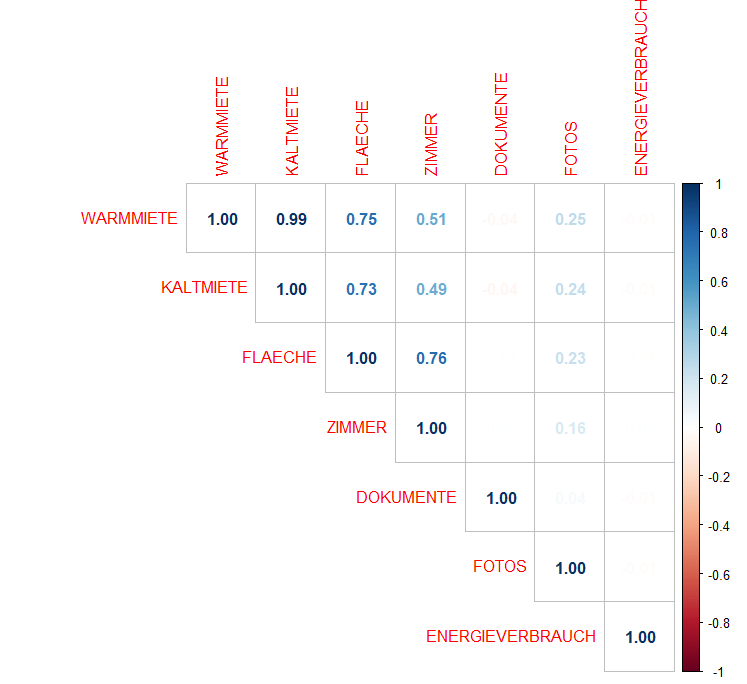
\includegraphics[width=0.7\linewidth]{img/korrelationVorher}
	\caption{Correlation plot before outlier analysis}
	\label{fig: korrelationVorher}
\end{figure}

It can be seen that the correlation between the warm rent and the cold rent is 99\% and that the area and the number of rooms show a very strong correlation with the rent price. This is plausible, since, as a rule, a larger apartment should also be more expensive. In addition, the correlation of almost 0 between the warm rent and energy consumption suggests that there could be erroneous data or outliers here. At this point, there could be a negative correlation, so that the rent becomes cheaper when the energy consumption is very high. Since the number of pages of this seminar paper is limited, not every feature will be discussed separately in the following. However, the problems that have arisen will be discussed using three examples. 


\subsection{Target variable warm and cold rent}

Based on the quantiles in table \ref{tbl: Quantile Warm- und Kaltmiete} and the fact that the range of rents is very large, it was decided to use a logarithmic representation in \ref{fig: log warm und kaltmiete}.

\begin{table}[H]
	\begin{verbatim}
		> summary(tbl$warmmiete)
		Min. 1st Qu.  Median    Mean 3rd Qu.    Max. 
		200     705    1021    1328    1614   19850 
		
		> summary(tbl$kaltmiete)
		Min. 1st Qu.  Median    Mean 3rd Qu.    Max. 
		72.0   519.8   793.2  1062.1  1303.7 17000.0 
	\end{verbatim}
	\caption{Quantiles of cold and warm rent}
	\label{tbl: Quantile Warm- und Kaltmiete}
\end{table}
In this chart, the so-called 'heavy tails' are clearly visible. There are some very low and very high rents that distort the plot. These data points were initially identified as outliers, but not yet removed so as not to influence the other characteristics in advance.

\begin{figure}[H]
	\subfigure[Cold rent]{\includegraphics[width=.45\linewidth]{"img/log kaltmiete"}}
	\subfigure[Warm rent]{\includegraphics[width=.45\linewidth]{"img/log warmmiete"}}
	\caption{Comparison of the cheapest and most expensive property }
	\label{fig: log warm und kaltmiete}
\end{figure}

\subsection{Area}

A part from the very strong correlation between the warm and cold rent, the highest correlation was recorded for the area. In the following, due to the high correlation between the warm and cold rent, only the warm rent is considered. Strange area values can also be seen for the area. The smallest property has an area of 7 $m^2$, the largest property is 706 $m^2$. These two properties were also marked as outliers. Figure  \ref{fig: fläche log warm} shows the root area and log warm rent including the outliers. It has been found that the adjusted $R^2$ has deteriorated in the logarithmic plot compared to the normal plot. It also showed that the $R^2$ of the root representation also deteriorated compared to the normal representation, but only minimally. Therefore, the root representation was initially chosen for the area.

\begin{figure}[H]
	\centering
	\includegraphics[width=0.7\linewidth]{img/fläche log warm}
	\caption{log warm rent and root area}
	\label{fig: fläche log warm}
\end{figure}


\subsection{Energy consumption, year of construction and energy class}

There are several problems for the features energy consumption, year of construction and energy class. First, there is some missing and incorrect data in the data and second, this analysis should ultimately be used to calculate a potential rental price for tenants or landlords. This results in the challenge that for a tenant, for example, the actual year of construction is not of interest, but a time period in which the property was built. Incorrect data also shows construction years from 0022, so data prior to 1700 was classified as missing data. To solve the problem of converting to a categorical variable, the KMEANS algorithm\footnote{\cite{KMEANS} S.8)} was used to calculate the optimal clusters. The missing data were then categorized as an additional category of 'Not specified'. This approach was applied to all three variables.
The figure \ref{fig: Baujahr Warmmiete boxplots} shows that the median warm rent increases as the age of the property increases.
\begin{figure}[H]
	\centering
	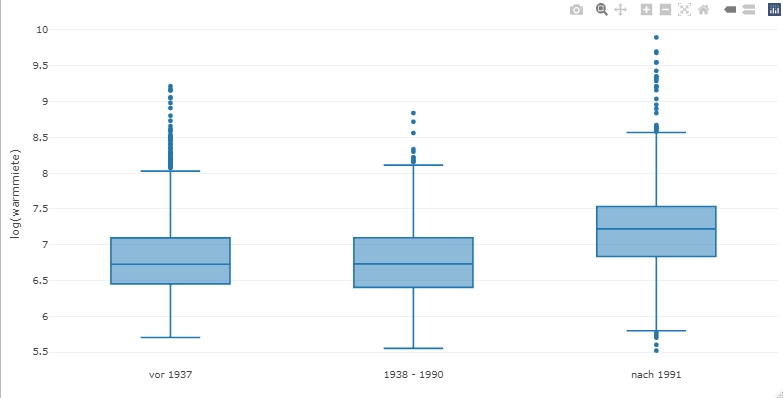
\includegraphics[width=0.7\linewidth]{img/Baujahr Warmmiete boxplots}
	\caption{Year of manufacture cluster boxplots}
	\label{fig: Baujahr Warmmiete boxplots}
\end{figure}
There are several reasons why the median warm rent might increase as the property ages. One possible reason could be that older buildings are usually less energy efficient and therefore incur higher energy costs, which can affect the rent price. Another reason could be that older buildings tend to be less modernized and therefore less attractive to tenants, which can also affect the rent price. It could also be that older buildings are simply in better locations or more popular neighborhoods and therefore have higher rents\footnote{At this point, further research could be conducted}.

\section{Interim summary}
Some interesting findings were obtained through the outlier analysis. On the one hand, it was found that the correlations between the numerical data were hardly improved by the different transformations (e.g. log or root representation). On the other hand, additional erroneous data came to light that had previously gone undetected. This erroneous data was classified as missing data and some features were transformed into categorical data. The Mahalonobis distance\footnote{For the mathematical basis be referred to \cite{Mahalonobis} and \cite{Mahalonobis2} Af page 325 and 326} was also calculated for the numerical data of warm rent, cold rent, area and number of rooms. This yielded 53 outliers, which are shown in Figure \ref{fig: Maha Ausreißer}.However, it turned out that the correlation between the variables nevertheless did not improve. 

\begin{figure}[H]
	\subfigure[Outlier log room and log price]{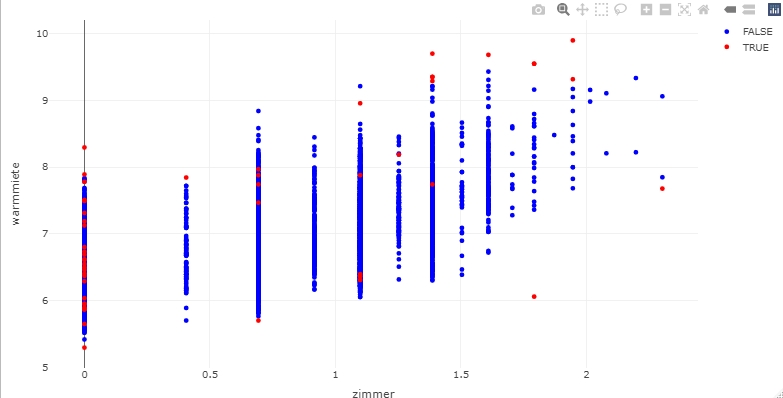
\includegraphics[width=0.3\linewidth]{img/maha zimmer Preis}}
	\subfigure[Outlier log area and log price]{\includegraphics[width=0.3\linewidth]{img/maha fläche Preis}}
	\subfigure[Outlier log area and log room]{\includegraphics[width=0.3\linewidth]{img/maha zimmer fläche}}
	\caption{Mahalanobis distance outlier}
	\label{fig: Maha Ausreißer}
\end{figure}
The correlations are shown in Figure \ref{fig: Korrelation nach der analyse}  dt can be seen that the correlation with energy consumption has improved signifikant. However, this is negligible because the data was transformed into a categorical variable. Also, the correlations for what are probably the most important features (area and room) have worsened rather than improved. For this reason, no outliers were ultimately removed. Nevertheless, the analysis was useful to correct erroneous data and stabilize the data set. With the entire 6520 data, development of various models will begin in Section 4. The correlation are shown in \ref{chapter: Modell}. 
\begin{figure}[h!]
	\centering
	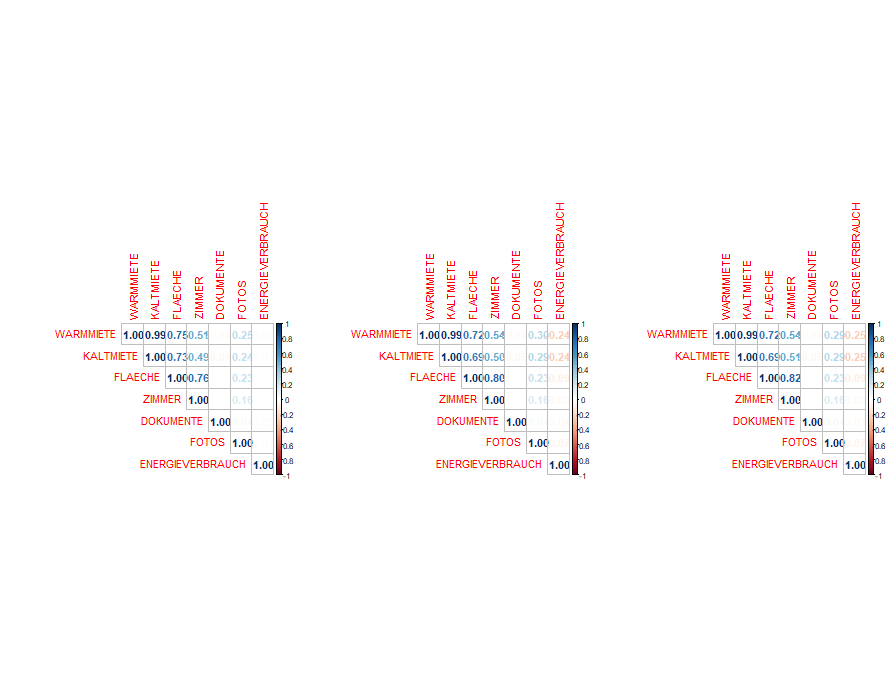
\includegraphics[width=0.9\linewidth]{img/Korrelation nach der analyse}
	\caption{Correlation plot after outlier analysis}
	\footnotesize\sffamily (Left before analysis, center log/root plot, right without outliers and log/root plot.) 
	\label{fig: Korrelation nach der analyse}
\end{figure}
